\documentclass[10pt]{standalone}
\usepackage{pgf,tikz,pgfplots}
\pgfplotsset{compat=1.15}
\usepackage{mathrsfs}
\usetikzlibrary{arrows}
\pagestyle{empty}
\begin{document}
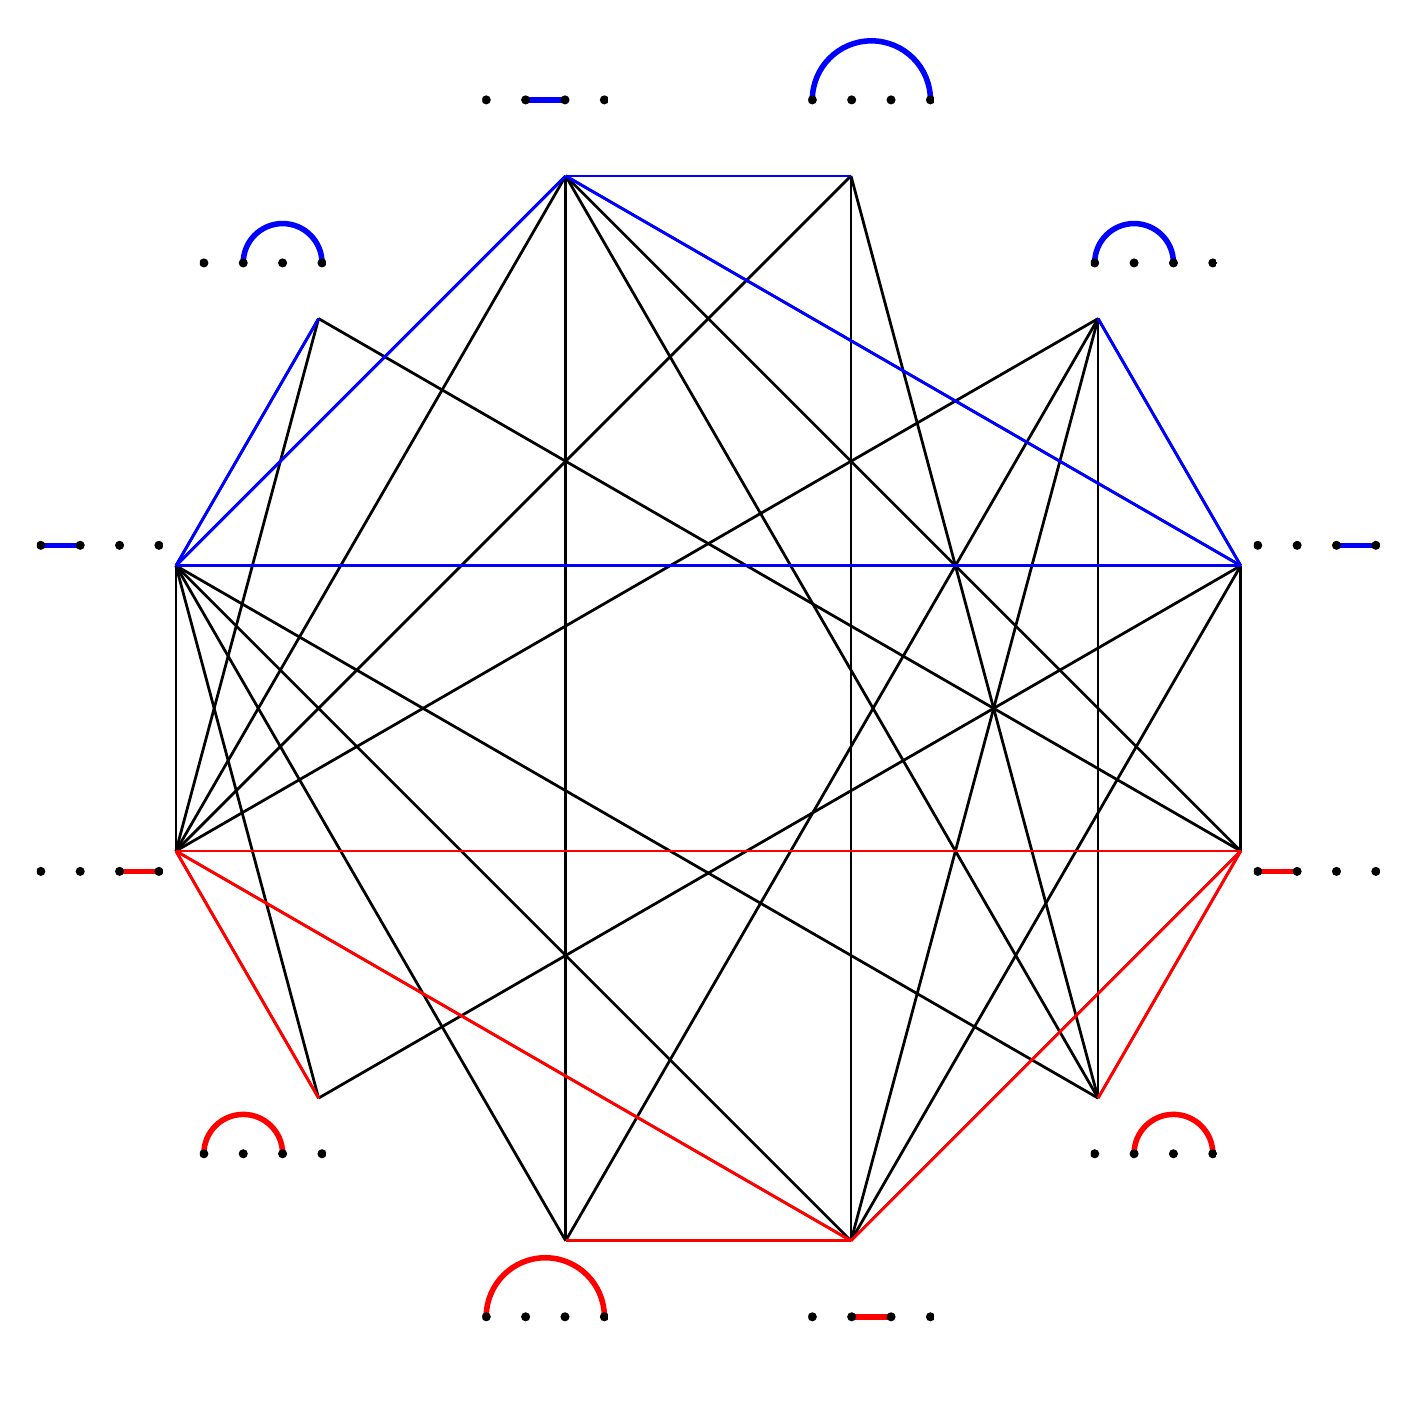
\begin{tikzpicture}

	\node () at (15:8) {\tikz[scale = 0.5]{
		\clip (1.5,0) circle (1.6);
		\draw[color =blue, line width = 2] (2, 0) -- (3, 0);
		\draw[fill = black] (0,0) circle (.1);
		\draw[fill = black] (1,0) circle (.1);
		\draw[fill = black] (2,0) circle (.1);
		\draw[fill = black] (3,0) circle (.1);
	}};
	\node (34b) at (15:7) {};
	
	\node () at (45:8) {\tikz[scale = 0.5]{
		\clip (1.5,0) circle (1.6);
		\draw[color =blue, line width = 2] (0, 0) arc (180:0:1.);
		\draw[fill = black] (0,0) circle (.1);
		\draw[fill = black] (1,0) circle (.1);
		\draw[fill = black] (2,0) circle (.1);
		\draw[fill = black] (3,0) circle (.1);
	}};
	\node (13b) at (45:7) {};
	
	\node () at (75:8) {\tikz[scale = 0.5]{
		\clip (1.5,0) circle (1.6);
		\draw[color =blue, line width = 2] (0, 0) arc (180:0:1.5);
		\draw[fill = black] (0,0) circle (.1);
		\draw[fill = black] (1,0) circle (.1);
		\draw[fill = black] (2,0) circle (.1);
		\draw[fill = black] (3,0) circle (.1);
	}};
	\node (14b) at (75:7) {};
	
	\node () at (105:8) {\tikz[scale = 0.5]{
		\clip (1.5,0) circle (1.6);
		\draw[color =blue, line width = 2] (1, 0) -- (2, 0);
		\draw[fill = black] (0,0) circle (.1);
		\draw[fill = black] (1,0) circle (.1);
		\draw[fill = black] (2,0) circle (.1);
		\draw[fill = black] (3,0) circle (.1);
	}};
	\node (23b) at (105.:7) {};
	
	\node () at (135:8) {\tikz[scale = 0.5]{
		\clip (1.5,0) circle (1.6);
		\draw[color =blue, line width = 2] (1, 0) arc (180:0:1.);
		\draw[fill = black] (0,0) circle (.1);
		\draw[fill = black] (1,0) circle (.1);
		\draw[fill = black] (2,0) circle (.1);
		\draw[fill = black] (3,0) circle (.1);
	}};
	\node (24b) at (135:7) {};
	
	\node () at (165:8) {\tikz[scale = 0.5]{
		\clip (1.5,0) circle (1.6);
		\draw[color =blue, line width = 2] (0, 0) -- (1, 0);
		\draw[fill = black] (0,0) circle (.1);
		\draw[fill = black] (1,0) circle (.1);
		\draw[fill = black] (2,0) circle (.1);
		\draw[fill = black] (3,0) circle (.1);
	}};
	\node (12b) at (165:7) {};
		
	\node () at (195:8) {\tikz[scale = 0.5]{
		\clip (1.5,0) circle (1.6);
		\draw[color =red, line width = 2] (2, 0) -- (3, 0);
		\draw[fill = black] (0,0) circle (.1);
		\draw[fill = black] (1,0) circle (.1);
		\draw[fill = black] (2,0) circle (.1);
		\draw[fill = black] (3,0) circle (.1);
	}};
	\node (34r) at (195:7) {};

	\node () at (225:8) {\tikz[scale = 0.5]{
		\clip (1.5,0) circle (1.6);
		\draw[color =red, line width = 2] (0, 0) arc (180:0:1.);
		\draw[fill = black] (0,0) circle (.1);
		\draw[fill = black] (1,0) circle (.1);
		\draw[fill = black] (2,0) circle (.1);
		\draw[fill = black] (3,0) circle (.1);
	}};
	\node (13r) at (225:7) {};

	\node () at (255:8) {\tikz[scale = 0.5]{
		\clip (1.5,0) circle (1.6);
		\draw[color =red, line width = 2] (0, 0) arc (180:0:1.5);
		\draw[fill = black] (0,0) circle (.1);
		\draw[fill = black] (1,0) circle (.1);
		\draw[fill = black] (2,0) circle (.1);
		\draw[fill = black] (3,0) circle (.1);
	}};
	\node (14r) at (255:7) {};
	
	\node () at (285:8) {\tikz[scale = 0.5]{
		\clip (1.5,0) circle (1.6);
		\draw[color =red, line width = 2] (1, 0) -- (2, 0);
		\draw[fill = black] (0,0) circle (.1);
		\draw[fill = black] (1,0) circle (.1);
		\draw[fill = black] (2,0) circle (.1);
		\draw[fill = black] (3,0) circle (.1);
	}};
	\node (23r) at (285:7) {};
	
	\node () at (315:8) {\tikz[scale = 0.5]{
		\clip (1.5,0) circle (1.6);
		\draw[color =red, line width = 2] (1, 0) arc (180:0:1.);
		\draw[fill = black] (0,0) circle (.1);
		\draw[fill = black] (1,0) circle (.1);
		\draw[fill = black] (2,0) circle (.1);
		\draw[fill = black] (3,0) circle (.1);
	}};
	\node (24r) at (315:7) {};
	
	\node () at (345:8) {\tikz[scale = 0.5]{
		\clip (1.5,0) circle (1.6);
		\draw[color =red, line width = 2] (0, 0) -- (1, 0);
		\draw[fill = black] (0,0) circle (.1);
		\draw[fill = black] (1,0) circle (.1);
		\draw[fill = black] (2,0) circle (.1);
		\draw[fill = black] (3,0) circle (.1);
	}};
	\node (12r) at (345:7) {};
	
	\draw[line width=1] (12b.center) -- (13r.center);
	\draw[line width=1] (12b.center) -- (14r.center);
	\draw[line width=1] (12b.center) -- (23r.center);
	\draw[line width=1] (12b.center) -- (24r.center);
	\draw[line width=1] (12b.center) -- (34r.center);
	\draw[line width=1] (13b.center) -- (14r.center);
	\draw[line width=1] (13b.center) -- (23r.center);
	\draw[line width=1] (13b.center) -- (24r.center);
	\draw[line width=1] (13b.center) -- (34r.center);
	\draw[line width=1] (14b.center) -- (23r.center);
	\draw[line width=1] (14b.center) -- (24r.center);
	\draw[line width=1] (14b.center) -- (34r.center);
	\draw[line width=1] (23b.center) -- (12r.center);
	\draw[line width=1] (23b.center) -- (14r.center);
	\draw[line width=1] (23b.center) -- (24r.center);
	\draw[line width=1] (23b.center) -- (34r.center);
	\draw[line width=1] (24b.center) -- (12r.center);
	\draw[line width=1] (24b.center) -- (34r.center);
	\draw[line width=1] (34b.center) -- (12r.center);
	\draw[line width=1] (34b.center) -- (13r.center);
	\draw[line width=1] (34b.center) -- (23r.center);
	\draw[line width=1, blue] (12b.center) -- (23b.center);
	\draw[line width=1, red] (12r.center) -- (23r.center);
	\draw[line width=1, blue] (12b.center) -- (24b.center);
	\draw[line width=1, red] (12r.center) -- (24r.center);
	\draw[line width=1, blue] (12b.center) -- (34b.center);
	\draw[line width=1, red] (12r.center) -- (34r.center);
	\draw[line width=1, blue] (13b.center) -- (34b.center);
	\draw[line width=1, red] (13r.center) -- (34r.center);
	\draw[line width=1, blue] (14b.center) -- (23b.center);
	\draw[line width=1, red] (14r.center) -- (23r.center);
	\draw[line width=1, blue] (23b.center) -- (12b.center);
	\draw[line width=1, red] (23r.center) -- (12r.center);
	\draw[line width=1, blue] (23b.center) -- (14b.center);
	\draw[line width=1, red] (23r.center) -- (14r.center);
	\draw[line width=1, blue] (23b.center) -- (34b.center);
	\draw[line width=1, red] (23r.center) -- (34r.center);
	\draw[line width=1, blue] (24b.center) -- (12b.center);
	\draw[line width=1, red] (24r.center) -- (12r.center);
	\draw[line width=1, blue] (34b.center) -- (12b.center);
	\draw[line width=1, red] (34r.center) -- (12r.center);
	\draw[line width=1, blue] (34b.center) -- (13b.center);
	\draw[line width=1, red] (34r.center) -- (13r.center);
	\draw[line width=1, blue] (34b.center) -- (23b.center);
	\draw[line width=1, red] (34r.center) -- (23r.center);

\end{tikzpicture}
\end{document}